\documentclass[tikz,border=15pt]{standalone}
\usepackage{tikz}
\usepackage{xcolor}
\usetikzlibrary{arrows.meta,calc,shapes.geometric}

\definecolor{bgcolor}{RGB}{15,23,42}
\definecolor{cardbg}{RGB}{30,41,59}
\definecolor{cardborder}{RGB}{51,65,85}
\definecolor{laserglow}{RGB}{239,68,68}
\definecolor{beamred}{RGB}{248,113,113}
\definecolor{interfererose}{RGB}{251,113,133}
\definecolor{cyanlight}{RGB}{56,189,248}
\definecolor{cyandark}{RGB}{2,132,199}
\definecolor{textblue}{RGB}{125,211,252}
\definecolor{amberlabel}{RGB}{251,191,36}
\definecolor{metalgray}{RGB}{203,213,225}
\definecolor{darkmount}{RGB}{71,85,105}
\definecolor{slategray}{RGB}{148,163,184}

\begin{document}
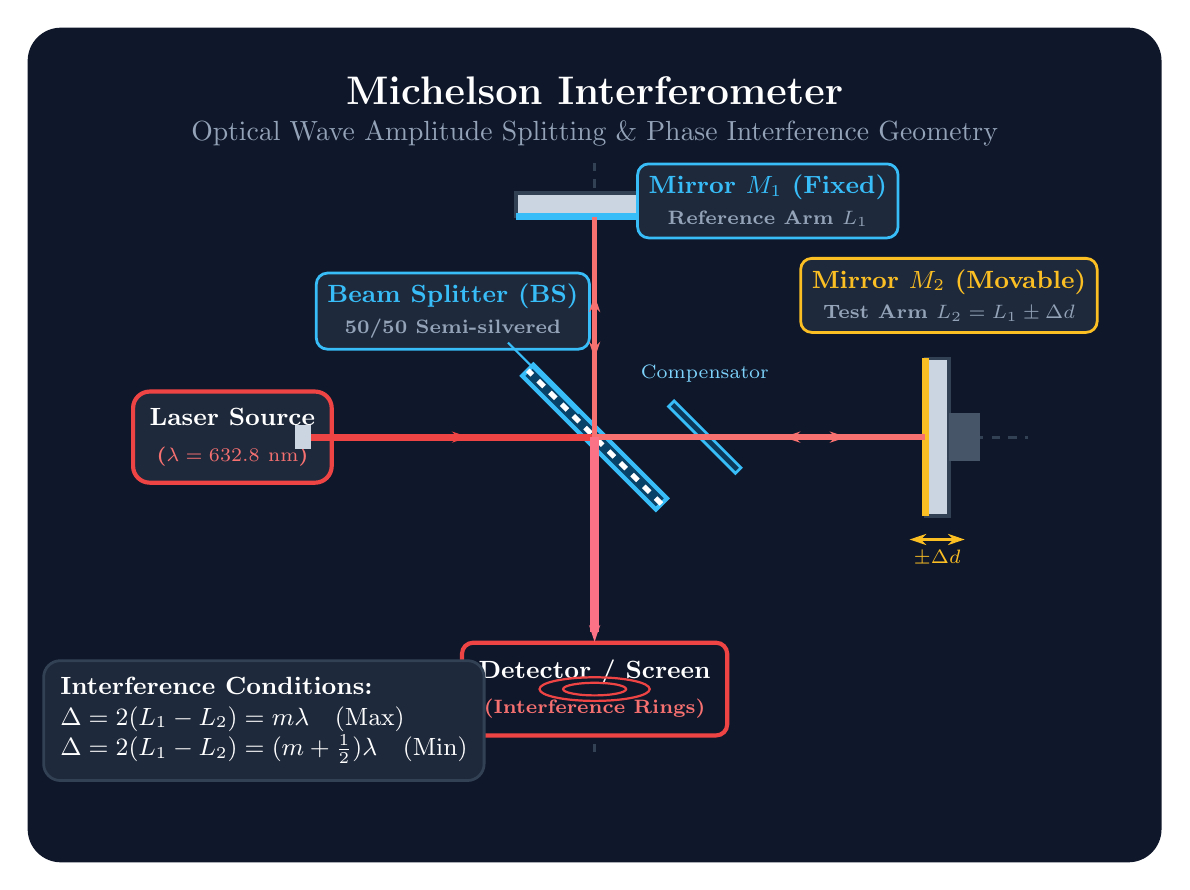
\begin{tikzpicture}[
    >={Stealth[length=6pt, width=4pt]}
]

% Background Card
\fill[rounded corners=12pt, fill=bgcolor] (-7.2,-5.4) rectangle (7.2,5.2);

% Title & Header
\node[text=white, font=\Large\bfseries] at (0, 4.4) {Michelson Interferometer};
\node[text=slategray, font=\normalsize] at (0, 3.85) {Optical Wave Amplitude Splitting \& Phase Interference Geometry};

% Optical Center at (0, 0)
\coordinate (O) at (0, 0);

% Optical Baselines (Dashed)
\draw[cardborder, dashed, line width=1pt] (-5.5, 0) -- (5.5, 0);
\draw[cardborder, dashed, line width=1pt] (0, -4.0) -- (0, 3.5);

% 1. LASER SOURCE (Left at -4.6, 0)
\node[fill=cardbg, draw=laserglow, line width=1.5pt, rounded corners=6pt, text=white, font=\small\bfseries, align=center, inner sep=6pt] (LASER) at (-4.6, 0) {
    Laser Source\\[2pt]
    \textcolor{beamred}{\scriptsize ($\lambda = 632.8\ \mathrm{nm}$)}
};
\fill[metalgray] (-3.8, -0.15) rectangle (-3.6, 0.15);

% 2. BEAM SPLITTER (Center, rotated 45 deg)
\fill[fill=cyandark, fill opacity=0.4, draw=cyanlight, line width=1.5pt, rotate around={45:(O)}] (-0.1, -1.2) rectangle (0.1, 1.2);
\draw[white, dashed, line width=1.8pt, rotate around={45:(O)}] (0, -1.2) -- (0, 1.2);

% Beam Splitter Callout
\node[fill=cardbg, draw=cyanlight, line width=1pt, rounded corners=4pt, text=cyanlight, font=\small\bfseries, align=center, inner sep=4pt] at (-1.8, 1.6) {
    Beam Splitter (BS)\\
    \textcolor{slategray}{\scriptsize 50/50 Semi-silvered}
};
\draw[cyanlight, line width=0.8pt] (-1.1, 1.2) -- (-0.2, 0.3);

% Compensator Plate
\fill[fill=cyandark, fill opacity=0.3, draw=cyanlight, line width=1pt, rotate around={45:(1.4, 0)}] (1.35, -0.6) rectangle (1.45, 0.6);
\node[text=textblue, font=\scriptsize] at (1.4, 0.8) {Compensator};

% 3. MIRROR M1 (Fixed Mirror, Top at 0, 2.8)
\fill[fill=metalgray, draw=cardborder, line width=1.2pt] (-1.0, 2.8) rectangle (1.0, 3.1);
\draw[cyanlight, line width=2.5pt] (-1.0, 2.8) -- (1.0, 2.8); % front surface
\node[fill=cardbg, draw=cyanlight, line width=1pt, rounded corners=4pt, text=cyanlight, font=\small\bfseries, align=center, inner sep=4pt] at (2.2, 3.0) {
    Mirror $M_1$ (Fixed)\\
    \textcolor{slategray}{\scriptsize Reference Arm $L_1$}
};

% 4. MIRROR M2 (Movable Mirror, Right at 4.2, 0)
\fill[fill=metalgray, draw=cardborder, line width=1.2pt] (4.2, -1.0) rectangle (4.5, 1.0);
\draw[amberlabel, line width=2.5pt] (4.2, -1.0) -- (4.2, 1.0); % front surface
\fill[darkmount] (4.5, -0.3) rectangle (4.9, 0.3);
\node[fill=cardbg, draw=amberlabel, line width=1pt, rounded corners=4pt, text=amberlabel, font=\small\bfseries, align=center, inner sep=4pt] at (4.5, 1.8) {
    Mirror $M_2$ (Movable)\\
    \textcolor{slategray}{\scriptsize Test Arm $L_2 = L_1 \pm \Delta d$}
};
\draw[amberlabel, <->, line width=1.2pt] (4.0, -1.3) -- (4.7, -1.3) node[midway, below, font=\scriptsize\bfseries] {$\pm \Delta d$};

% 5. DETECTOR & SCREEN (Bottom at 0, -3.2)
\node[fill=bgcolor, draw=laserglow, line width=1.5pt, rounded corners=4pt, text=white, font=\small\bfseries, align=center, inner sep=6pt] (DET) at (0, -3.2) {
    Detector / Screen\\[2pt]
    \textcolor{beamred}{\scriptsize (Interference Rings)}
};
% Rings preview on detector
\draw[laserglow, line width=0.8pt] (0, -3.2) ellipse (0.7cm and 0.15cm);
\draw[laserglow, line width=0.8pt] (0, -3.2) ellipse (0.4cm and 0.08cm);

% 6. LIGHT BEAM PATHS
% Laser to BS
\draw[laserglow, line width=2.5pt] (-3.6, 0) -- (O);
\draw[laserglow, line width=2pt, ->] (-2.8, 0) -- (-1.6, 0);

% Split to M1 (Up and Down)
\draw[beamred, line width=2pt] (O) -- (0, 2.8);
\draw[beamred, line width=1.5pt, ->] (0, 0.8) -- (0, 1.8);
\draw[beamred, line width=1.5pt, ->] (0, 2.0) -- (0, 1.0);

% Split to M2 (Right and Left)
\draw[beamred, line width=2pt] (O) -- (4.2, 0);
\draw[beamred, line width=1.5pt, ->] (2.2, 0) -- (3.2, 0);
\draw[beamred, line width=1.5pt, ->] (3.4, 0) -- (2.4, 0);

% Recombined Beam to Detector
\draw[interfererose, line width=3.5pt, ->] (O) -- (0, -2.6);

% 7. INTERFERENCE FORMULAS BOX
\node[fill=cardbg, draw=cardborder, line width=1pt, rounded corners=6pt, text=white, font=\small, align=left, inner sep=6pt] at (-4.2, -3.6) {
    \textbf{Interference Conditions:}\\
    $\Delta = 2(L_1 - L_2) = m\lambda\quad \mathrm{(Max)}$\\
    $\Delta = 2(L_1 - L_2) = (m+\frac{1}{2})\lambda\quad \mathrm{(Min)}$
};

\end{tikzpicture}
\end{document}
